\chapter{การสำรวจข้อมูล}
\section{Dataset Description}
Dataset สำหรับการ Train มีทั้งหมด 454 แถว 3 คอลลัมน์ ประกอบด้วย:
\begin{enumerate}
    \item Title ชื่อของงานวิจัย
    \item Abstract บทคัดย่อ
    \item Classes ป้ายกำกับสาขาของงานวิจัยนั้น
\end{enumerate}

ทำการโหลดไฟล์ train.json เข้า Pandas Dataframe
\begin{figure}[ht]
    \centering
    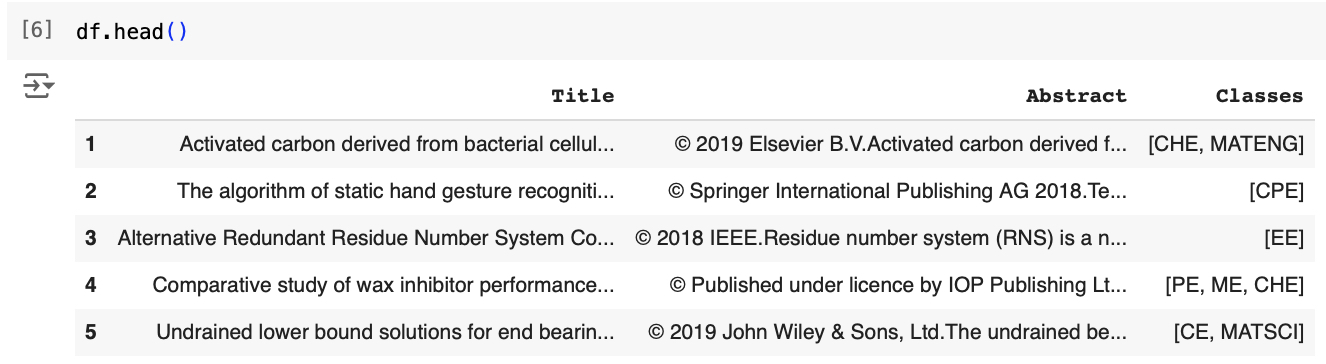
\includegraphics[width=\imgwidth]
    {images/dataframe_head.jpg}
    \caption{ตัวอย่าง Dataframe}
    \label{fig:dataframe_head}
\end{figure}
\clearpage


\begin{figure}
    \centering
    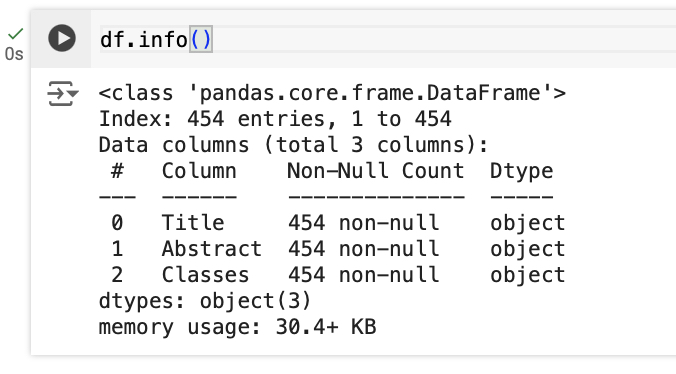
\includegraphics[width=\imgwidth]
    {images/dataframe_info.jpg}
    \caption{รายละเอียด Dataframe}
    \label{fig:dataframe_info}
\end{figure}
รายละเอียด Dataframe ประกอบด้วย 454 แถว และ 3 คอลลัมน์
\section{Data Statistics}
ดูการกระจายตัวของข้อมูลแต่ละคลาส พบว่าคลาสไม่่สมดุลกัน โดยที่คลาสที่มีมากที่สุดคือ CHE มีจำนวนมากถึง 177 แถวและคลาสที่มีจำนวนน้อยที่สุดคือ AGRI มีเพียง 20 แถว ดังนั้นจะต้องคำนวณ class weight เพื่อทำไปใช้ใน loss function
\begin{figure}[ht]
    \centering
    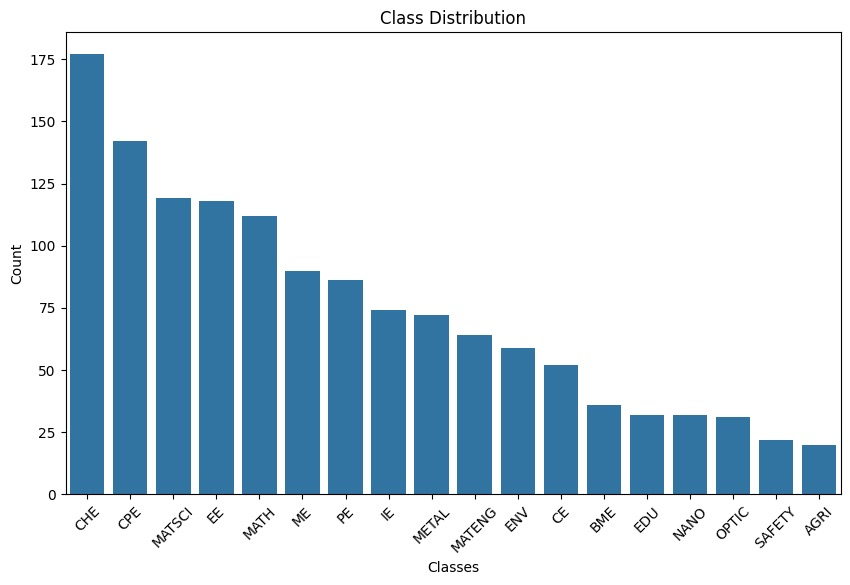
\includegraphics[width=\imgwidth]
    {images/class_distribution.jpg}
    \caption{การกระจายตัวของแต่ละ class}
    \label{fig:class_distribution}
\end{figure}


\section{Data Preprocessing}
การเตรียมข้อมูลประกอบด้วย แปลงให้ตัวอักษรเป็น lower case ลบตัวอักษรพิเศษ ลบเลข ลบช่องว่างที่ไม่จำเป็น และลดรูปคำให้เหลือเพียงคำฐานโดยใช้ spacy library \cite{spacy2}
\begin{figure}[ht]
    \centering
    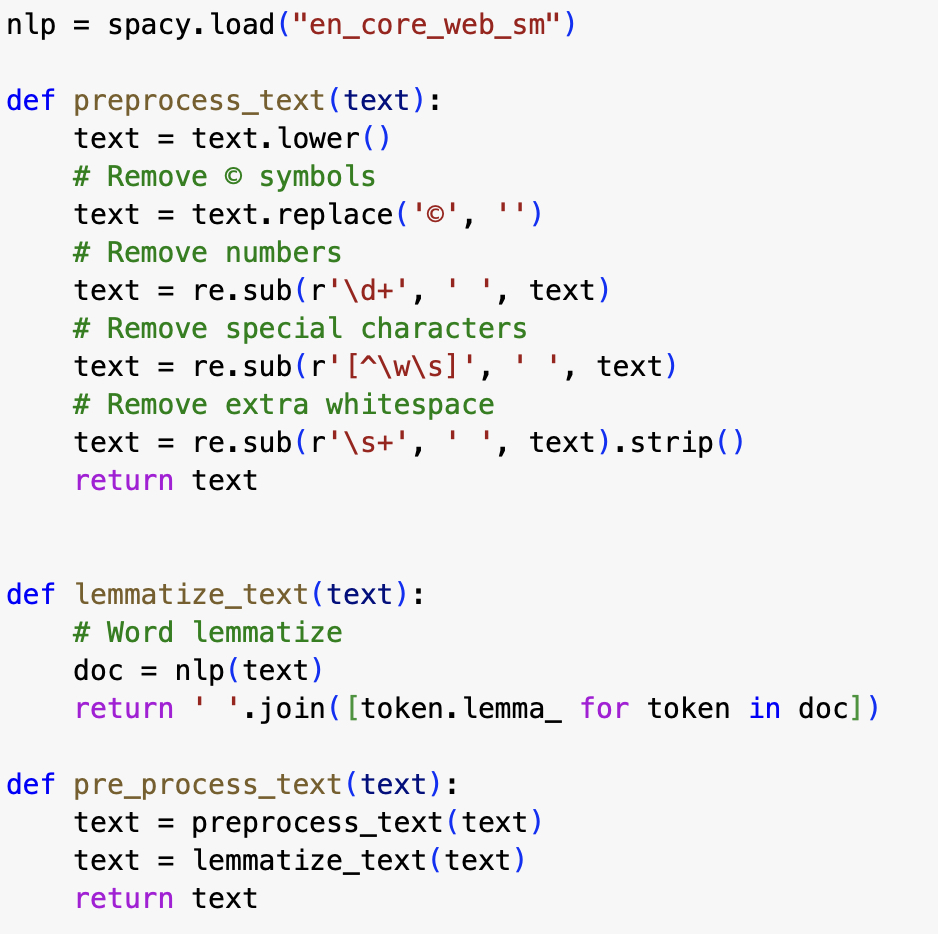
\includegraphics[width=\imgwidth]
    {images/preprocess.jpg}
    \caption{การ Preprocess Data}
    \label{fig:preprocess}
\end{figure}


หลังจากนั้นทำการแปลง Label ของข้อมูลให้เป็นรูปแบบ Binary ด้วย MultiLabelBinarizer จาก library scikit-learn \cite{pedregosa2011scikit}

\begin{figure}[ht]
    \centering
    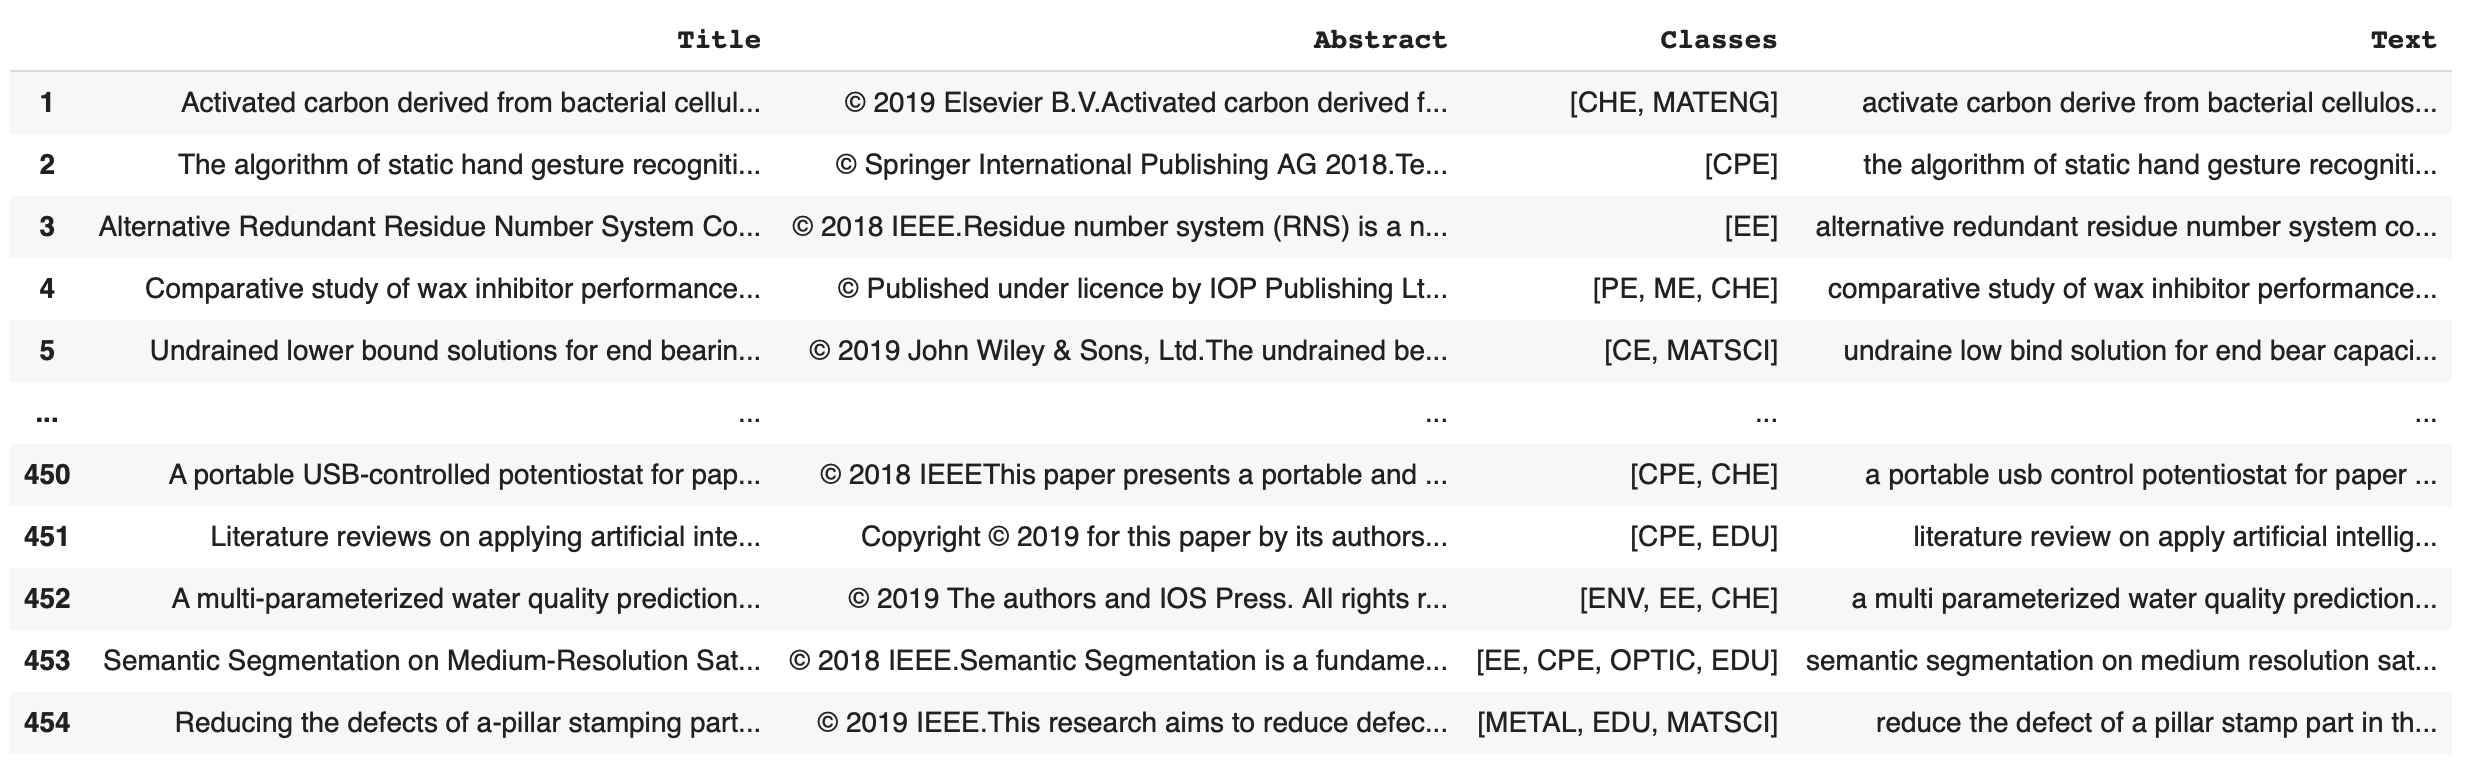
\includegraphics[width=\imgwidth]
    {images/dataframe_after_preprocessed.jpg}
    \caption{ข้อความที่อยู่ในคอลัมน์ Text เป็นข้อความที่ผ่านการ Preprocess แล้ว}
    \label{fig:dataframe_after_preprocessed}
\end{figure}